\documentclass[a4paper]{article}

%% Language and font encodings
\usepackage[english]{babel}
\usepackage[utf8x]{inputenc}
\renewcommand{\baselinestretch}{1.5}
\usepackage[T1]{fontenc}
\usepackage{graphicx}

%% Sets page size and margins
\usepackage[letterpaper,top=3cm,bottom=2cm,left=3cm,right=3cm,marginparwidth=1.75cm]{geometry}

%% Useful packages
\usepackage{amssymb} 
\usepackage{placeins}
\usepackage{amsmath}
%%%%%%%%%%%%%%%%%%%%%%%%%%%%%%%%%%%%%%%%%%%%%%%%%%%%%%%%%%%%%%%%%%%%%%%%%%%%
\begin{document}
\begin{titlepage}

\centering
\paragraph*{\huge \linebreak\linebreak \linebreak Continuum Mechanics Overview}


\paragraph*{ \large MechE 287\linebreak \linebreak \normalsize Taught by Prof. Casey\linebreak Mechanical Engineering Department\linebreak\linebreak  \linebreak \linebreak\linebreak \linebreak \linebreak \linebreak \large \linebreak \linebreak \linebreak \linebreak\linebreak \linebreak Author \linebreak \linebreak \normalsize  Brian Howell}

\paragraph*{\linebreak \linebreak \large Date \normalsize \linebreak \linebreak Fall Semester 2019}

\end{titlepage}

\pagebreak
%\tableofcontents
%\listoffigures


\pagebreak

\pagebreak
%%%%%%%%%%%%%%%%%%%%%%%%%%%%%%%%%%%%%%%%%%%
\section{Introduction}
This overview of MechE 287 is essentially a commentary review of Prof. Casey's course on Continuum Mechanics and follows the important ideas of the subject by walking through example problems from the homework. Assignments through out the document are referred to as $\mathbf{A_i}$ while problems are referred to as $\mathbf{P_i}$. Peridically, sections are directly copied Panos' notes, as well as notes for Material Point Method for Simluating Continuum Materials by Joseph Teran. This review is by no means my own work, rather a compilation of material for a quick reminder on the subject. 


\section{Kinematics and Deformation}

The main idea of continuum mechanics the description of the deformation and kinematics of a material. The two analogous ideas here being the deformation gradient $\mathbf{F}$ and the velocity gradient $\mathbf{L}$.

\subsection{Deformation}
In continuum mechanics, the deformation is usually represented with the material (or undeformed space $\boldsymbol{\mathcal{X}}$, the world (or deformed) space $\boldsymbol{\chi}$ and a deformation map $\phi(\boldsymbol{\mathcal{X}},t)$. You can simply treat $\boldsymbol{\mathcal{X}}$ as the "initial position" and $\boldsymbol{\chi}$ as the "current position" for any point in the simulated material. In particular, at time $t=0$, $\boldsymbol{\mathcal{X}}$ and $\boldsymbol{\chi}$ have the same value (Jiang et al. p.11). 

Here is a more detailed definition. We consider the motion of material to be determined by mapping $\phi (\cdot, t): \Omega^0 \xrightarrow{} \Omega^t$ for $\Omega^0, \Omega^t \subset \mathbb{R}^d$ where $d = 2$ or $3$ is the dimension of the simulated material (or domain). The mapping $\phi$ is sometimes called the flow map or the deformation map. POints in the set $\Omega^0$ are referred to as material points and are denoted as $\boldsymbol{\mathcal{X}}$. Points in $\Omega^t$ represent the location of material points at time t. They are referred to as $\boldsymbol{\chi}$. In other words, $\phi$ describes the motion of each material point $\boldsymbol{\mathcal{X}} \subset \Omega^0$ over time (Jiang et al. p.11):

\begin{equation}\label{eq:1}
    \boldsymbol{\chi} = \boldsymbol{\chi}(\boldsymbol{\mathcal{X}}, t) = \phi(\boldsymbol{\mathcal{X}},t).
\end{equation}

Consider the $\mathbf{A3}$ $\mathbf{P1}$ part (a) where the motion $\boldsymbol{\mathcal{X}}$ of a deformable continuum $\mathcal{B}$ is described in component form on a single or fixed orthonormal basis: 

\begin{equation}\label{eq:2}
    x_1 = e^tX_1, \quad x_2 = X_2 + t, \quad x_3 = e^{-t}X_3
\end{equation}

Note that $\mathcal{B}$ occupies the reference configuration at at $t=0$. 
The material deforms along the basis provided by the motion listed in Eq. \ref{eq:2}. However, since the motion does not change to the same extent in all directions, the concept of the deformation gradient becomes useful for computing the relative deformation. Commonly referred as $\mathbf{F}$, the deformation gradient can be represented in component form as $\mathbf{F} = Grad (\boldsymbol{\chi}) = \boldsymbol{\chi_{i,A}} \mathbf{e_i} \otimes \mathbf{E_A}$ and is often referred to as the Jacobina of the deformation map. In tensor form, the motion listed in Eq \ref{eq:2} can be represented as: 

\begin{equation}
    [F_{i,A}] = 
    \begin{bmatrix}
    \frac{dx_1}{dX_1} & \frac{dx_1}{dX_2} & \frac{dx_1}{dX_3} \\
    \frac{dx_2}{dX_1} & \frac{dx_2}{dX_2} & \frac{dx_2}{dX_3} \\
    \frac{dx_3}{dX_1} & \frac{dx_3}{dX_2} & \frac{dx_3}{dX_3}
  \end{bmatrix} = 
  \begin{bmatrix}
    e^t & 0 & 0 \\
    0 & 1 & 0 \\
    0 & 0 & e^{-t}
  \end{bmatrix}
\end{equation}

The deformation of a material may result in a change in volume. This change in volume (often referred to as $J$) can be computed by taking the determinant of $J = det\mathbf{F}$ where $J<1$ indicates a decrease in volume, $J>1$ indicates an increase in volume, and $J=1$ indicates a no change in volume. Note that for rigid body motion $J=1$. 

\subsection{Eulerian and Lagrangian Descriptions}

An important concept in continuum mechanics the reference frame for which deformations are represented. This is particularly important when taking into consideration the velocity field of a motion. The Lagrangian perspective is observed from the initial location of a material point, while the Eulerian perspective makes observation from the current configuration. 

An applied example of this is the difference between true and engineering stress. Consider a tensile specimen undergoing a traction force. The stress experience within test portion of the dogbone is computed by $\sigma = \frac{t_n}{area}$. The typical method for obtaining this area is to measure the initial area prior to testing and to compute an "engineering stress" based off of the initial state. In reality, the specimen will exhibit necking, or a change in area. This means that the true stress should contain an updating area for an accurate measure of what is occurring within the material. In this example, the Lagrangian description is analogous to the engineering stress while the Eulerian description is analogous to the true stress. 

\begin{figure}[ht!]
\centering
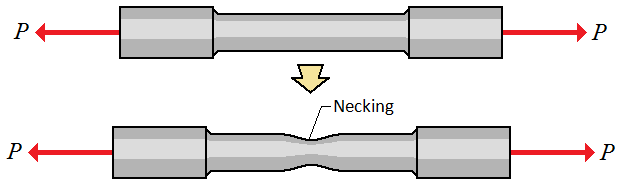
\includegraphics[width=0.6\textwidth]{engineering_stress.png}
\caption{\label{fig:engineering_stress}True vs. Engineering Stress}
\end{figure}
\FloatBarrier

Once again, consider the motion described in $\mathbf{A3}$ $\mathbf{P1}$ (Eq. \ref{eq:2}). A velocity field can be computed in both the Lagrangian and Eulerian descriptions. 

\begin{equation}
    \text{Lagrangian:} \quad [\mathbf{\hat{v}}] = \mathbf{\dot{x}}(\mathbf{X},t) = 
    \begin{bmatrix}
      e^t X_1 \\
      1 \\
      -e^{-1}X_3
    \end{bmatrix}
\end{equation}

The Eulerian description can be determined by solving deformation map $\phi$ for $\mathbf{X}$ and plugging into the Lagrangian description. 

\begin{equation}
    \text{Eulerian:} \quad [\mathbf{\Tilde{v}}] = \mathbf{\dot{X}}(\mathbf{x},t) = 
    \begin{bmatrix}
      e^t e^{-t}x_1 \\
      1 \\
      -e^{-1}e^tx_3
    \end{bmatrix}
    =
    \begin{bmatrix}
      x_1 \\
      1 \\
      -x_3
    \end{bmatrix}
\end{equation}

Both are equally valid ways of examining the motion, but we generally work with the Eulerian description for other applications. 

\subsection{The Material Derivative}
The time-rate of change of the velocity field is not nearly as straight forward as the deformation gradient. The Eulerian description of the acceleration field is a little bit different. Since the current configuration is also changing with time, the velocity field is actually a function of two functions and there for the chain rule is required. 
 
 \begin{equation}
     \Tilde{\mathbf{a}} = \frac{\partial \mathbf{v}}{\partial t}(\phi(\mathbf{X},t),t) + \frac{\partial \mathbf{v}}{\partial \mathbf{x}}(\phi(\mathbf{X}),t) \frac{\partial \phi}{\partial t}(\mathbf{X},t) = \frac{\partial \mathbf{v}}{\partial t}(\phi(\mathbf{X},t),t) + \frac{\partial \mathbf{v}}{\partial t}(\phi(\mathbf{X},t),t) \hat{\mathbf{v}}
 \end{equation}
 
 For example consider a velocity field which is given in the the spatial (or Eulerian) form (see midterm problem 2b) by: 

\begin{equation}
    \hat{v}_1 = \frac{\partial \psi}{\partial x_2}, \quad \hat{v}_2 = -\frac{\partial \psi}{\partial x_1}, \quad \hat{v}_3 = 0
\end{equation}

where 

\begin{equation}
    \psi(x_1, x_2) = \frac{1}{2}\omega(x_1^2 + x_2^2), \quad \omega = \text{const}. 
\end{equation}
 
 Therefore the acceleration field (in the Eulerian description) is then given by:
 
\begin{align}
    \Tilde{a}_1 &= \frac{\partial \Tilde{v}_1}{\partial t} + \frac{\partial \Tilde{v}_1}{\partial x_1} \frac{\partial x_1}{\partial t} + \frac{\partial \Tilde{v}_1}{\partial x_2} \frac{\partial x_2}{\partial t} + \frac{\partial \Tilde{v}_1}{\partial x_3} \frac{\partial x_3}{\partial t} \\
                &= 0 + 0 + (\omega)(-\omega x_1) + 0 \\
                &= -\omega^2 x_1
\end{align}

\begin{align}
    \Tilde{a}_2 &= \frac{\partial \Tilde{v}_2}{\partial t} + \frac{\partial \Tilde{v}_2}{\partial x_1} \frac{\partial x_1}{\partial t} + \frac{\partial \Tilde{v}_2}{\partial x_2} \frac{\partial x_2}{\partial t} + \frac{\partial \Tilde{v}_2}{\partial x_3} \frac{\partial x_3}{\partial t} \\
                &= 0 + (-\omega)(\omega x_2) + 0 + 0 \\
                &= -\omega^2 x_2
\end{align}

\begin{align}
    \Tilde{a}_2 &= \frac{\partial \Tilde{v}_3}{\partial t} + \frac{\partial \Tilde{v}_3}{\partial x_1} \frac{\partial x_1}{\partial t} + \frac{\partial \Tilde{v}_3}{\partial x_2} \frac{\partial x_2}{\partial t} + \frac{\partial \Tilde{v}_3}{\partial x_3} \frac{\partial x_3}{\partial t} \\
                &= 0 + 0 + 0 + 0 \\
                &= 0
\end{align}

Although the relationship between the Eulerian $\mathbf{a}$ and $\mathbf{v}$ is not simply via partial differentiation with respect to time, the relationship is a common one and it is often called the material derivative (Jiang pg. 15). The notation

\begin{equation}
    \frac{D}{Dt}v_i(\mathbf{x},t) = \frac{\partial v_i}{\partial t} + \frac{\partial v_i}{\partial x_j}(\mathbf{x},t) v_j(\mathbf{x},t)
\end{equation}

\subsection{Stretch}
In addition to the change in volume caused by a deformation, the stretch of a vector within the material is also of interest. The stretch $\lambda$ of the infinitesimal material line element $d\mathbf{X}$ and $d\mathbf{x}$ at time $t$ is defined as 

\begin{equation}
    \lambda = \frac{ds}{dS}
\end{equation}

and also noting that $d\mathbf{x} = \mathbf{F}d\mathbf{X} = \mathbf{F} \mathbf{M} dS$. Thus

\begin{equation}
    \lambda \mathbf{m} = \mathbf{F} \mathbf{M}
\end{equation}

Where $\mathbf{M}$ is a unit vector in reference configuration and $\mathbf{m}$ is that same unit vector in the current configuration. Often it is difficult to $\mathbf{m}$. One way around this is to dot multiply each side by itself (see Panos pg. 45) to get 

\begin{equation}
    \lambda^2 = \mathbf{M} \cdot \mathbf{F}^T \mathbf{F} \mathbf{M}
\end{equation}

\subsection{Right Cauchy-Green Deformation Tensor}
The sequence $\mathbf{F}^T \mathbf{F}$ in Eq. 8 is actually a commonly used tensor. In fact, it has has its own name, the Right Cauchy-Green Deformation Tensor, or $\mathbf{C} = \mathbf{F}^T \mathbf{F}$, or in component form $C_{AB} = F_{iA}F_{iB}$. It is important to observe that $\mathbf{C}$ is  symmetric and positive-definite, and is defined with respect to the basis in the reference configuration. Conversely, we can obtain a similar tensor that is defined by the basis of the current configuration, or also referred to as the left Cauchy-Green tensor, $\mathbf{B} = \mathbf{F}\mathbf{F}^T$, or in component form $B_{ij} = F_{iA}F_{jA}$.  

Recall from $\mathbf{A4}$ $\mathbf{P1}$ the motion:

\begin{equation}
    x_1 = \frac{3}{\sqrt{2}} X_1 - \frac{5}{\sqrt{2}} X_2, \quad x_2 = \frac{3}{\sqrt{2}} X_1 + \frac{5}{\sqrt{2}} X_2, \quad
    x_3 = X_3
\end{equation}
 
We can compute the right Cauchy-Green Tensor by first computing the deformation gradient and then computing $\mathbf{C} = \mathbf{F}^T \mathbf{F}$.

\begin{equation*}
    [C_{AB}] = 
    \begin{bmatrix}
      \frac{3}{\sqrt{2}} & \frac{3}{\sqrt{2}} & 0 \\
      - \frac{5}{\sqrt{2}} & \frac{5}{\sqrt{2}} & 0 \\
      0 & 0 & 1
    \end{bmatrix}
    \begin{bmatrix}
      \frac{3}{\sqrt{2}} & - \frac{5}{\sqrt{2}} & 0 \\
      \frac{3}{\sqrt{2}} & \frac{5}{\sqrt{2}} & 0 \\
      0 & 0 & 1
    \end{bmatrix}
    =
    \begin{bmatrix}
      9 & 0 & 0 \\
      0 & 25 & 0 \\
      0 & 0 & 1
    \end{bmatrix}
\end{equation*}


\subsection{Lagrangian \& Eulerian Strain Tensors}
The strain within a material is often measure of interest. Consider the difference between $ds^2 - dS^2$ in the square of the length of the line element $d\mathbf{X}$ and $d\mathbf{x}$: 

\begin{equation}
    ds^2 - dS^2 = d\mathbf{x} \cdot d\mathbf{x} - d\mathbf{X} \cdot d\mathbf{X} = d\mathbf{X} \cdot 2\mathbf{E}d\mathbf{X}
\end{equation}

where 

\begin{equation}
    \mathbf{E} = \frac{1}{2} (\mathbf{C} - \mathbf{I}). 
\end{equation}

The full derivation can be found in Panos pg 48. $\mathbf{E}$ in equation 11 is the (relative) Lagrangian strain tensor, and in component form $E_{AB} = \frac{1}{2} (C_{AB} - \delta_{AB})$. This shows that the Lagrangian Strain Tensor $\mathbf{E}$ is defined with respect to the basis in the reference configuration. In addition $\mathbf{E}$ is clearly symmetric and vanishes when the body undergoes no deformation between the reference and current configuration (Panos pg. 49) 
The Eulerian strain tensor is also derived in Panos' notes and only the final relationship is shown here. 

\begin{equation}
    e_{ij} = \frac{1}{2} (\delta_{ij} - B^{-1}_{ij})
\end{equation}

Like $\mathbf{E}$, the tensor $\mathbf{e}$ is symmetric and vanishes when the current configuration remains the undeformed relative to the reference configuration. However, unlike $\mathbf{e}$ is naturally resolved into components on the basis in the current configuration. 

\subsection{Polar Decomposition}

While in general the infinitesimal material line element $d\mathcal{X}$ is is both stretched and rotated due to $\mathbf{F}$, neither $\mathbf{C}$, $\mathbf{B}$, $\mathbf{E}$, nor $\mathbf{e}$ yield any useful information regarding the rotation of $d\mathbf{X}$. To extract rotation-related information from $\mathbf{F}$, recall the polar decomposition theorem, which states that any invertible tensor $\mathbf{F}$ can be uniquely decomposed into 

\begin{equation}\label{eqn 27}
    \mathbf{F} = \mathbf{R} \mathbf{U} = \mathbf{V} \mathbf{R}, 
\end{equation}

where $\mathbf{R}$ is an orthogonal tensor and $\mathbf{U}$, $\mathbf{V}$ are symmetric positive-definite tensors. The symmetric matrices contain the information for only the stretching of the linear transformation. In fact, the eigenvalues the symmetric matrix are always positive. The rotation matrix contains all other information with regards to rotation, inversion, etc. It is also important to note that $\mathbf{R}$ is an orthogonal matrix. This means that the columns and rows of the tensor are orthogonal unit vector. This means that $\mathbf{R}^T \mathbf{R} = \mathbf{I}$ and that $\mathbf{R}^T = \mathbf{R}^{-1}$. Also note that determinate of any orthogonal tensor is always either $+1$ or $-1$. In component form, the polar decomposition is expressed as 

\begin{equation}
    F_{iA} = R_{iB}U_{BA} = V_{ij}R_{jA}. 
\end{equation}

The following relationships should prove useful:

\begin{equation}
    \mathbf{C} = \mathbf{U}^2
\end{equation}

\begin{equation}
    \mathbf{B} = \mathbf{V}^2
\end{equation}

In $\mathbf{A4}$ $\mathbf{P1}$ part c, we computed $\mathbf{U}$. 
\begin{equation*}
    [U_{AB}] = [C_{AB}^{1/2}] = 
    \begin{bmatrix}
      \sqrt{9} & 0 & 0 \\
      0 & \sqrt{25} & 0 \\
      0 & 0 & \sqrt{1}
    \end{bmatrix}
    = 
    \begin{bmatrix}
      3 & 0 & 0 \\
      0 & 5 & 0 \\
      0 & 0 & 1
    \end{bmatrix}
\end{equation*}
\subsection{Velocity Gradient and Other Measures of Deformation}

Generally, we will take into consideration motions that imply deformations in the form of fields. In euclidean space, this implies motions for the directions of $\mathbf{e_1}$, $\mathbf{e_2}$, $\mathbf{e_3}$. For example ($\mathbf{A_2}$, $\mathbf{P_3}$), consider a velocity field of a continuum $\mathcal{B}$ with the Eulerian description of: 

\begin{equation*}
    v_1 = ax_1x_2^2, \quad v_2 = -b x_1^2 x_2, \quad v_3 = c x_3 t^2 . 
\end{equation*}

where $a$, $b$, and $c$ are constants. This field implies movements for any point within the continuum in the Euclidean space. However, there are some important things to note about such a velocity field. Notice that $v_1$ and $v_2$ are not functions of time and are there for constant. Although the derivatives with respect to time are zero, the derivatives with respect to $x_1$ and $x_2$ are not zero. This would imply that there is a velocity gradient within the the material. This velocity gradient is called $\mathbf{L}$, which can be compactly represented as:

\begin{equation}
    \mathbf{L} = v_{i,j} \mathbf{e_i}\otimes\mathbf{e_j}
\end{equation}

Determining the velocity gradient $\mathbf{L}$ can be explicitly computed as:

\begin{equation*}
    [L_{ij}] = 
    \begin{bmatrix}
    v_{1,1} & v_{1,2} & v_{1,3} \\
    v_{2,1} & v_{2,1} & v_{2,1} \\
    v_{3,1} & v_{3,2} & v_{3,3}
  \end{bmatrix} = 
  \begin{bmatrix}
    a x_2^2 & 2 a x_1 x_2 & 0 \\
    -2 b x_1 x_2 & -b x_1^2 & 0  \\
    0 & 0 & c t^2 
  \end{bmatrix}
\end{equation*}

Within this matrix $\mathbf{L}$, more information can be extracted by applying polar decomposition. Recall that any tensor can be uniquely decomposed into a symmetric and skew-symmetric part, so that $\mathbf{L}$ can be written as (Panos pg. 66): 

\begin{equation}\label{eqn 31}
    \mathbf{L} = \mathbf{D} + \mathbf{W}
\end{equation}

where 

\begin{equation}
    \mathbf{D} = \frac{1}{2}(\mathbf{L} + \mathbf{L}^T)
\end{equation}

is that rate-of-deformation tensor, which is symmetric, and

\begin{equation}
    \mathbf{W} = \frac{1}{2}(\mathbf{L} - \mathbf{L}^T)
\end{equation}

is the vorticity (or spin) tensor, which is skew-symmetric. 

Another point that should be examined is the time-rate of change of the deformation gradient for fixed particle associated with $\mathbf{X}$ in the reference configuration. To this end, write the material derivative of $\mathbf{F}$ as 

\begin{equation}\label{eqn 34}
    \dot{\mathbf{F}} = \dot{\overline{\biggl(\frac{\partial\boldsymbol{\chi}(\mathbf{X},t)}{\partial \mathbf{X}}\biggr)}} = \frac{\partial}{\partial \mathbf{X}} \dot{\overline{\boldsymbol{\chi}(\mathbf{X},t)}} = \frac{\partial \hat{\mathbf{v}}(\mathbf{X},t)}{\partial \mathbf{X}} = \frac{\partial \Tilde{\mathbf{v}}(\mathbf{x},t)}{\partial \mathbf{x}} \frac{\partial \boldsymbol{\chi}(\mathbf{X},t)}{\partial \mathbf{X}} = \mathbf{L} \mathbf{F}
\end{equation}

\section{Jacobian of the Deformation Gradient}

Consider a small piece of a material of unit volume in the reference configuration defined by the basis $e_1, e_2, e_3$. Now consider a differential stretch $dS$ in each direction where $dS = d\mathbf{X}^1$ in the $e_1$ direction, $dS = d\mathbf{X}^2$ in the $e_2$ direction and $dS = d\mathbf{X}^3$ in the $e_3$ direction. Since the material is of unit size, the volume is simple to compute and is just $V = dS^3$. 

\begin{figure}[ht!]
    \centering
    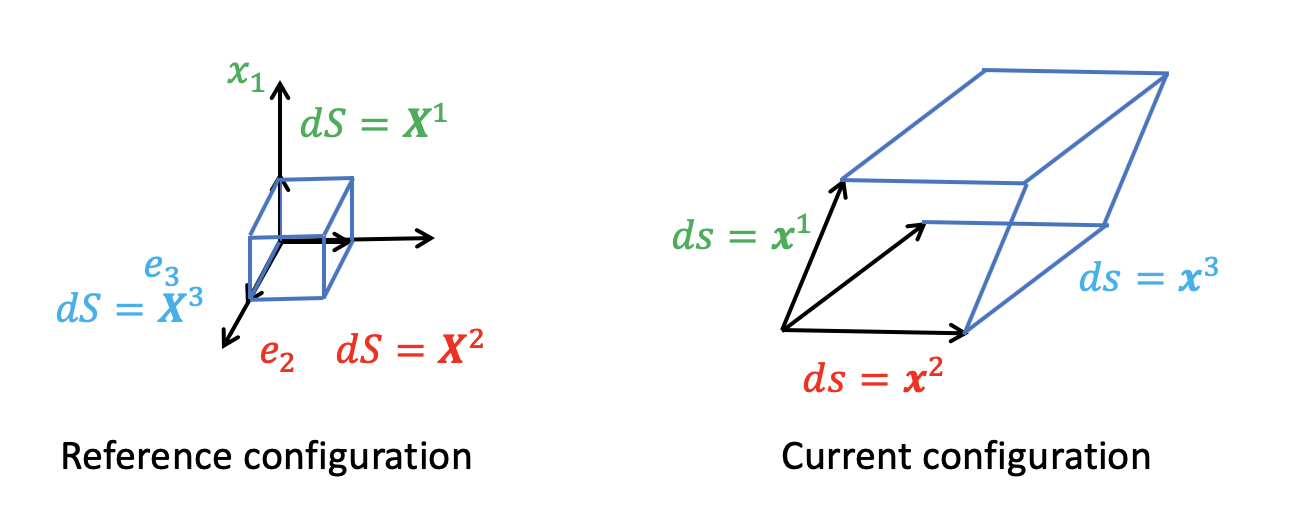
\includegraphics[width=0.8\textwidth]{infinitesimal_deformation.png}
    \caption{Infinitesimal deformation in the reference and current configurations. }
    \label{fig:infinitesimal_deformation}
\end{figure}

Now consider a deformation on that same small piece of material in the current configuration. The infinitesimal deformation can now be composed in the directions of $x_1, x_2,x_3$ where the stretch $ds = d\mathbf{x}$. The volume of in the current configuration can be determined by taking the triple scalar product which is defined as $d\mathbf{x}^{(1)} \cdot \biggl(d\mathbf{x}^{(2)} \times d\mathbf{x}^{(3)} \biggr)$. The cross product between two vectors computes the area and dot product extends the area in that vectors direction and gives the volume of the parallel piped. This triple scalar product returns a rank 2 tensor  as shown below. 

\begin{equation}
    d\Omega = 
    d\mathbf{x}^{(1)} \cdot \biggl(d\mathbf{x}^{(2)} \times d\mathbf{x}^{(3)} \biggr) = \begin{bmatrix}
    dx_{1}^{(1)} & dx_{2}^{(1)} & dx_{3}^{(1)} \\
    dx_{2}^{(1)} & dx_{2}^{(2)} & dx_{2}^{(1)} \\
    dx_{3}^{(1)} & dx_{3}^{(1)} & dx_{3}^{(1)}
  \end{bmatrix}
\end{equation}

Recall that previously we defined $dS = d\mathbf{X}^1 = d\mathbf{X}^2 = d\mathbf{X}^3$ and that $\mathbf{F} = \frac{\partial \mathbf{x}}{\partial \mathbf{X}} \rightarrow \partial \mathbf{x} = \mathbf{F} \cdot \partial \mathbf{X}$. Rearranging these equations yields

\begin{equation}\label{eqn:36}
    \begin{bmatrix}
    dx_{1}^{(1)} & dx_{2}^{(1)} & dx_{3}^{(1)} \\
    dx_{2}^{(1)} & dx_{2}^{(2)} & dx_{2}^{(1)} \\
    dx_{3}^{(1)} & dx_{3}^{(1)} & dx_{3}^{(1)}
    \end{bmatrix} = 
    \begin{bmatrix}
     \frac{\partial x_1}{\partial X_1} dS & 
     \frac{\partial x_2}{\partial X_1} dS & 
     \frac{\partial x_3}{\partial X_1} dS \\
     \frac{\partial x_1}{\partial X_2} dS & 
     \frac{\partial x_2}{\partial X_2} dS &
     \frac{\partial x_3}{\partial X_2} dS\\
    \frac{\partial x_1}{\partial X_3} dS & 
    \frac{\partial x_2}{\partial X_3} dS & 
    \frac{\partial x_1}{\partial X_1} dS
    \end{bmatrix}. 
\end{equation}

Now recall that $\text{det}(cA) = c^n \text{det}(A)$ for an $n\times n$ matrix $A$ and that $\text{det}(A^T) = \text{det}(A)$. Therefore the Eqn \ref{eqn:36} can be reduced to 

\begin{equation}
    \begin{bmatrix}
     \frac{\partial x_1}{\partial X_1} dS & 
     \frac{\partial x_2}{\partial X_1} dS & 
     \frac{\partial x_3}{\partial X_1} dS \\
     \frac{\partial x_1}{\partial X_2} dS & 
     \frac{\partial x_2}{\partial X_2} dS &
     \frac{\partial x_3}{\partial X_2} dS\\
    \frac{\partial x_1}{\partial X_3} dS & 
    \frac{\partial x_2}{\partial X_3} dS & 
    \frac{\partial x_1}{\partial X_1} dS
    \end{bmatrix} = 
    \text{det}(\mathbf{F^T}) dS^3 = \text{det}(\mathbf{F})dS^3
\end{equation}

The determinant of $\mathbf{F}$ is referred to as the Jacobian of the deformation gradient and indicates the change in volume.

\begin{equation}
    \text{det}(\mathbf{F}) dS^3 = J (dS^3) = J |d\Omega_0| = |d\Omega|^*
\end{equation}

*(refers to volume of the domain)


We now have a relationship between the volumes of the reference and current configurations as determined by $J$. This can be extend to other properties such as density. Consider the conservation of mass through the integral of the density throughout a volume

\begin{equation}
    \int_{\Omega_0} \rho_0 d\Omega_0 = \int_{\Omega} \rho d\Omega = \int_{\Omega_0} \rho J d\Omega_0 = mass. 
\end{equation}

Now that we have the relationship $\int_{\Omega_0} \rho_0 d\Omega_0 = \int_{\Omega_0} \rho J d\Omega_0$ where the bounds of integration are now the same, we can use the \textit{localization theorem} to draw the final relationship 

\begin{equation}\label{eqn:40}
    \boxed{\rho J = \rho_0 \rightarrow J = \frac{\rho_0}{\rho}}
\end{equation}

\section{Balance of Momentum/Equilibrium}

\begin{figure}[ht!]
    \centering
    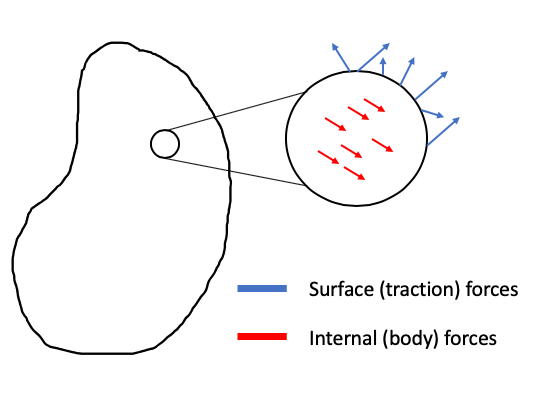
\includegraphics[width=0.6\textwidth]{traction_body_forces.png}
    \caption{Classes of forces that act on a piece of material.}
    \label{fig:forces}
\end{figure}
\FloatBarrier

Recall Newton's third law of motion; To every action there is always opposed an equal reaction: or the mutual actions of two bodies upon each other are always equal, and directed to contrary parts. If we consider a piece of material that is undergoing some sort of stress or strain, we can classify the internal forces that are being into two different categories: surfaces (traction) forces or internal (body) forces (see Fig. \ref{fig:forces}). Recall Newton's third law of motion; To every action there is always opposed an equal reaction: or the mutual actions of two bodies upon each other are always equal, and directed to contrary parts. Considering the consequences of the summation of all traction forces and body forces, the results in a motion or change of momentum in of the mass. Traction forces can be considered any type of force that is applied the surface of the material (e.g., wind, piston etc). Eqn \ref{eqn:41} shows summation of each of the classes of forces being equal to the change in momentum. 

\begin{equation}\label{eqn:41}
    \int_{\partial \omega} \mathbf{t} dA + \int_{\omega} \mathbf{f} d\omega = \frac{d}{dt} \int_{\omega} \rho \dot{\mathbf{u}} d\omega 
\end{equation}

Note the bounds of integration for each of the three terms. The first term on the left-hand side integrates all of the traction vectors over the boundary of the domain ($\partial \omega$) for a total surface area $A$. The traction vectors have units of $force/area$ and are multiplied with the total surface area once the integral has been performed resulting in a term with units of force. The second term integrates all of the body forces over the entire domain $\omega$. The momentum term on the right hand side also integrates momentum over the entire domain $\omega$. However, since the forces add up to the change in momentum, this term needs to have a differential term (with respect to time) in front. This differential term cannot transcend the integral since the domain might be changing with time (deformation or non-rigid body motions results in a change in the domain size which may result in an increase or decrease in volume). 

Eqn \ref{eqn:41} is fairly difficult to work with in this form. However, by examining each term we can simplify it into something much easier to compute. First let's consider the  term on the right hand side. We know from the conservation of mass that $\rho_0 = \rho J \rightarrow J d\omega_0 = d\omega$. Therefore

\begin{equation}
    \frac{d}{dt}\int_\omega \rho \dot{\mathbf{u}} d\omega = \frac{d}{dt}\int_{\omega_0} \rho \dot{\mathbf{u}} J d\omega_0 = \frac{d}{dt} \int_{\omega_0} \rho_0 \dot{\mathbf{u}} d\omega_0 .
\end{equation}

Now that the momentum term has bounds of integration within the reference configuration, the differential term can transcend the integral and operate on $\rho_0 \dot{\mathbf{u}}$ which results in

\begin{equation}
    \frac{d}{dt} \int_{\omega_0} \rho_0 \dot{\mathbf{u}} d\omega_0 =  \int_{\omega_0} \rho_0 \ddot{\mathbf{u}} d\omega_0. 
\end{equation}

Using the Jacobian relationship once again, we can change the bounds of integration back to the current configuration in the force balance in Eqn \ref{eqn:41}. 

\subsection{Cauchy Tetrahedron}
The first term on the left hand side of Eqn \ref{eqn:41} is also some what difficult to deal with. However, it is important to explore what these traction vectors are actually doing on the piece of material. This is typically done by introducing the Cauchy Tetrahedron which is essentially a small volume in the reference configuration (unit side lengths and volume). 

However, we know that the traction force $\mathbf{t} = \boldsymbol{\sigma}^T \cdot \mathbf{n} = \boldsymbol{\sigma} \cdot \mathbf{n}$ (later derived in section on the Cauchy Tetrahedron). Since this is a surface integral over a vector, we can use the divergence theorem


\section{Viscoelastic Flow}

This section goes over the re-derivation of Daniel Ram's paper Material Point Method for Viscoelastic Fluids, Foams and Sponges. The model consists of the governing equations: a material balance, a momentum balance, and plastic flow. 

\subsection{The Governing Equations}

\subsubsection{The Continuity Equation}

Matter cannot be made or destroyed , and so the total mass of a fluid element must remain the same. Thus if the density of a fluid element decreases, its volume must expand accordingly. This expansion causes a divergence of the velocity field, giving the conservation equation

\begin{equation}
    \frac{D}{Dt} \rho 
    = \frac{\partial}{\partial t} \rho + \frac{\partial \rho}{\partial x} \frac{\partial x}{\partial t} + \frac{\partial \rho}{\partial y} \frac{\partial y}{\partial t} + \frac{\partial
    \rho}{\partial z} \frac{\partial z}{\partial t} 
\end{equation}

\begin{equation}\label{eq. 36}
    \boxed{0 = \frac{\partial \rho}{\partial t} + \mathbf{v} \cdot \nabla \rho }
\end{equation}

If the density of the fluid is constant, approximately true of most liquid including water, then Eq. \ref{eq. 36} reduces to 

\begin{equation}
    \nabla \cdot \mathbf{v} = 0 
\end{equation}

\subsubsection{Momentum balance}

Imagine for an infinitesimally small voxel of fluid moving within a flow field. This voxel carries with it a computable momentum. Any change in the momentum will cause the particle to accelerate as a result of a sum of forces on that voxel of material. Mathematically, this can also be seen as a force balance. 

\begin{equation}
    \boxed{\rho \frac{D}{Dt}\mathbf{v} = \nabla \cdot \boldsymbol{\sigma} + g \mathbf{g}}
\end{equation}

\subsubsection{Cauchy Stress}
The first term on the right hand side contains the gradient of the Cauchy stress applied to the material. Just as shown in Eqn. \ref{eqn 31}, the Cauchy stress can be further broken down into different components that take into account different material properties of the fluid in question, in this case, the fluid (Newtonian) aspect of the fluid and the elastic portion of the fluid. 

\begin{equation}
    \boldsymbol{\sigma} = \boldsymbol{\sigma}^N +  \boldsymbol{\sigma}^E
\end{equation}

 The Newtonian part of the Cauchy stress tensor is similar to that of the rate-of-deformation tensor $\mathbf{D}$, which takes into account the rate at which the material is deforming. Just like $\mathbf{D}$, $\boldsymbol{\sigma}^N$ is defined as
 
\begin{equation}
    \boldsymbol{\sigma}^N = \frac{\mu^N}{2}\biggl(\frac{\partial \mathbf{v}}{\partial \mathbf{x}} + \frac{\partial \mathbf{v}}{\partial \mathbf{x}}^T \biggr) = \frac{\mu^N}{2}\biggl(\mathbf{L} + \mathbf{L}^T \biggr)
\end{equation}
 
The elastic portion is of of the Cauchy stress tensor is expressed as 
 
\begin{equation}
     \boldsymbol{\sigma}^E = \frac{2}{J}\frac{\partial \psi}{\partial \mathbf{B}^E} \mathbf{B}^e. 
\end{equation}

\subsubsection{Polar Decomposition of the Deformation Gradient}
The constitutive behaviour of the elastic component can be expressed by decomposing the the deformation gradient $\mathbf{F}$. However, rather than describing the decomposition as rotating and stretching tensors as in Eqn \ref{eqn 27}, the deformation gradient is decomposed into tensors that describe the elastic and plastic components of the deformation. 

\begin{equation}\label{eqn 42}
    \mathbf{F} = \mathbf{F}^E \mathbf{F}^P
\end{equation}

At this point, it is important to note the direction of this derivation. The plastic flow is predefined as the time differential of the right Cauchy-Green strain tensor $\frac{D}{Dt}\mathbf{C}^P$. The way this is computed is by examining the elastic portion of the deformation gradient. Consider the modification of Eqn \ref{eqn 42}

\begin{equation}\label{eqn 43}
    \mathbf{F}^E = \mathbf{F} (\mathbf{F}^P)^{-1}. 
\end{equation}

Now consider the left elastic Cauchy-Green strain tensor with Eqn \ref{eqn 43} plugged in and reduced

\begin{align}
    \mathbf{B}^E 
    &= \mathbf{B}^E (\mathbf{B}^E)^T \\
    &= \mathbf{F} (\mathbf{F^P})^{-1} [\mathbf{F} (\mathbf{F}^P)^{-1}]^T \\
    &= \mathbf{F} (\mathbf{F}^P)^{-1} ((\mathbf{F}^P)^T)^{-1} \mathbf{F}^T\\
    &= \mathbf{F} \biggl[((\mathbf{F}^P)^T) (\mathbf{F}^P) \biggr]^{-1} \mathbf{F}^T \\ 
    &= \mathbf{F} [\mathbf{C}^P]^{-1} \mathbf{F}^T
\end{align}

Recall that the left elastic Cauchy-Green strain tensor takes into account the deformation in the Eulerian or current configuration. What we are looking for is the time rate of a change of this deformation, which results in the material undergoing plastic flow. This can be obtained by taking the material derivative of $\mathbf{B}^E$. 

\begin{equation}\label{eqn 49}
    \frac{D}{Dt}\mathbf{B}^E = \frac{D}{Dt}\mathbf{F} (\mathbf{C}^P)^{-1} \mathbf{F}^T + \mathbf{F}(\mathbf{C})^{-1} \frac{D}{Dt} \mathbf{F}^T + \mathbf{F} \frac{D}{Dt}(\mathbf{C}^P)^{-1} \mathbf{F}^T
\end{equation}

Recall from Eqn \ref{eqn 34} that the material derivative of the deformation gradient is $\mathbf{F} = \mathbf{L} \mathbf{F}$ and that the definition of the left elastic Cauchy-Green strain tensor is given by $\mathbf{B}^E = \mathbf{F} (\mathbf{C}^P)^{-1} \mathbf{F}^T$. Therefore Eqn \ref{eqn 49}, can be further simplified as 

\begin{align}label{eqn 52}
    \frac{D}{Dt}\mathbf{B}^E 
    &= \mathbf{L} \mathbf{F} (\mathbf{C}^P)^{-1} \mathbf{F}^T + \mathbf{F} (\mathbf{C}^P)^{-1} [\mathbf{L} \mathbf{F}]^T + \mathbf{F} \frac{D}{Dt}(\mathbf{C}^P)^{-1} \mathbf{F}^T \\
    &= \mathbf{L} \mathbf{F} (\mathbf{C}^P)^{-1} \mathbf{F}^T + \mathbf{F} (\mathbf{C}^P)^{-1} \mathbf{F}^T \mathbf{L}^T + \mathbf{F} \frac{D}{Dt}(\mathbf{C}^P)^{-1} \mathbf{F}^T \\
    &= \mathbf{L}\mathbf{B}^E + \mathbf{B}^E \mathbf{L}^T + \mathbf{F} \frac{D}{Dt}(\mathbf{C}^P)^{-1} \mathbf{F}^T
\end{align}

Notice that there is now a term on the right hand side that that has a time differential of the right elastic Cauchy-Green strain tensor, or the plastic flow term. In this Ram's paper, they let this term be 

\begin{equation}\label{eqn 53}
    \mathop{\mathbf{B}}^\nabla\limits{}^{E} = g(\mathbf{B}^E) = \mathbf{F} \frac{D}{Dt}(\mathbf{C}^P)^{-1} \mathbf{F}^T. 
\end{equation}

The final description for the plastic flow term $\mathbf{F} \frac{D}{Dt}(\mathbf{C}^P)^{-1} \mathbf{F}^T$ is now

\begin{equation}
    \mathop{\mathbf{B}}^\nabla\limits{}^{E} = \mathbf{F} \frac{D}{Dt}(\mathbf{C}^P)^{-1} \mathbf{F}^T = \frac{D}{Dt} \mathbf{B}^E - \mathbf{L}\mathbf{B}^E - \mathbf{B}^E \mathbf{L}^T 
\end{equation}

At this point in the paper, Ram introduces the Oldroyd-B constitutive equation relating the plasticity term $g(\mathbf{B}^E)$ to the left elastic Cauchy-Green strain tensor. 

\begin{equation}
    g(\mathbf{B}^E) = \frac{1}{W_i}(\mathbf{I} - \mathbf{B}^E)
\end{equation}

The damping of the plasticity is taken into account with the Weissenberg number, $W_i$ -- the larger the damping the less impact the plasticity term as on the overall governing equations. Equating the Oldroyd-B Equation to Eqn \ref{eqn 53} yields 

\begin{equation}
    \mathbf{F} \frac{D}{Dt}(\mathbf{C}^P)^{-1} \mathbf{F}^T = \frac{1}{W_i}(\mathbf{I} - \mathbf{B}^E). 
\end{equation}

Solving for the differential form of $\mathbf{C}^P$ 

\begin{equation}
    \frac{D}{Dt} [(\mathbf{C}^P)^{-1}] = \frac{1}{W_i}[(\mathbf{C})^{-1} - (\mathbf{C}^P)^{-1}]
\end{equation}

where $\mathbf{C} = \mathbf{F}^T \mathbf{F}$ is the right Cauchy-Green strain tensor. The purpose of deriving this term with the Oldroyd-B model is that it is computationally easier for implicit time stepping.

\subsubsection{Incompressible flow}

Unfortunately, the Oldroyd model does not inherently exhibit isochoric features (more specifically, the $det(\mathbf{F}) \neq 1$). To address this issue, as slight modification to the Oldroyd model needs to be made. Consider the modified $\mathbf{B}_{OB}^E$ strain tensor

\begin{equation}
    \mathbf{B}^E \equiv \biggl(\frac{J}{J_{OB}}\biggr)^{\frac{2}{3}} \mathbf{B}^E_{OB}
\end{equation}

where $J = \text{det}(\mathbf{F}$ and $J_{OB} = \sqrt{\text{det}(\mathbf{B}_{OB}^E})$. 

This modification to the Oldroyd plasticity obeys

\begin{equation}
    \mathop{\mathbf{B}}^\nabla\limits{}^{E} = \frac{D}{Dt}\Biggl( \biggl(\frac{J}{J_{OB}}\biggr)^{2/3}\Biggr) \mathbf{B}^E_{OB} + \frac{1}{W_i}\biggl(\frac{J}{J_{OB}}\biggr) (\mathbf{I} - \mathbf{B}_{OB}^E )
\end{equation}

which can be further solved to give the plastic flow

\begin{equation}\label{eqn 60}
    \frac{d}{dt} \mathbf{F}^{-1}\mathbf{F} (\mathbf{C}^P) \mathbf{F}^T\mathbf{F}^{-T} = \frac{d}{dt}\Biggr[\biggl(\frac{J}{J_{OB}}\biggl)^{2/3}\Biggr] \mathbf{F}^{-1} \mathbf{B}_{OB}^E \mathbf{F}^{-T} + \frac{1}{W_i}\biggl(\frac{J}{J_{OB}}\biggr)^{2/3} \biggr[\mathbf{C}^{-1} - \mathbf{F}^{-1} \mathbf{B}_{OB}^E \mathbf{F}^{-T}\biggr]. 
\end{equation}

Recall that $\mathbf{B}_{OB}^{-1} = \mathbf{F} \biggl(\mathbf{C}_{OB}^P \biggr)^{-1} \mathbf{F}^T$, Eqn \ref{eqn 60} becomes

\begin{equation}
    \boxed{\frac{d}{dt} \mathbf{F}^{-1}\mathbf{F} (\mathbf{C}^P) \mathbf{F}^T\mathbf{F}^{-T} = \frac{d}{dt}\Biggr[\biggl(\frac{J}{J_{OB}}\biggl)^{2/3}\Biggr] \biggl(\mathbf{C}_{OB}^P \biggr)^{-1} + \frac{1}{W_i}\biggl(\frac{J}{J_{OB}}\biggr)^{2/3} \biggr[\mathbf{C}^{-1} - \mathbf{C}_{OB}^{-1}\biggr]}
\end{equation}

which is the plastic flow for an incompressible fluid. 

\subsubsection{Neo-Hookean Elastic Potential Energy Density}
In this paper, the constitutive behaviour is described by the compressible Neo-Hookean elastic potential energy density. The general form is given in Jiang Pg. 19 is represented by

\begin{equation}
    \psi(\mathbf{B}^E) = \frac{\mu}{2}(\text{tr}(\mathbf{F}^T \mathbf{F}) - d) - \mu \text{log}(J) + \frac{\lambda}{2}\textit{log}^2(J). 
\end{equation}

where $d=2$ or 3 denotes the problem dimension, $\mu$ and $\lambda$ are related to Young's modulus and $E$ and Poisson's ratio $\nu$ via 

\begin{equation}
    \mu = \frac{E}{2*1+\nu}, \quad \lambda = \frac{E \nu}{(1+\nu)(1-2\nu)}
\end{equation}

If the deformation gradient $\mathbf{F}$ consists of only rotation, it is easy to see that Eq 62 reduces to $\psi 
(\mathbf{F}) = 0$ ($E = 0$, $J = 0$). 

In the context of Ram's paper, Eqn 62 is reduced to 

\begin{equation}
    \psi(\mathbf{B}^E) = \frac{\mu}{2}(\text{tr}(\mathbf{B}^E) - 3) - \mu \text{ln}(J) + \frac{\lambda}{2}(J-1)^2
\end{equation}

Plugging this equation into the Eqn 41 and differentiating yields

\begin{equation}
    \boldsymbol{\sigma}^E = \frac{\mu}{J}(\mathbf{B}^E-\mathbf{I}) + \lambda (J-1)\mathbf{I}
\end{equation}

\end{document}
